\fancyhead{}
\fancyhead[L]{\textbf{\textsf{20}}\qquad \textbf{\textsf{CHƯƠNG 1}}\quad Các hàm số và Mô hình}
\enlargethispage{\baselineskip}
\noindent
\begin{multicols}{2}
\fontsize{8pt}{9.8pt}\selectfont
\setlength{\abovedisplayskip}{1pt}
\setlength{\belowdisplayskip}{1pt}

\noindent
\textbf{\color{stewartcyan}39--46}\quad \textbf{Tìm tập xác định của hàm số.}

\vspace{3pt}
\noindent
\textbf{39.} $f(x) = \dfrac{x + 4}{x^2 - 9}$ \hfill \textbf{40.} $f(x) = \dfrac{x^2 + 1}{x^2 + 4x - 21}$

\vspace{2pt}
\noindent
\textbf{41.} $f(t) = \sqrt[3]{2t - 1}$ \hfill \textbf{42.} $g(t) = \sqrt{3 - t} - \sqrt{2 + t}$

\vspace{2pt}
\noindent
\textbf{43.} $h(x) = \dfrac{1}{\sqrt[4]{x^2 - 5x}}$ \hfill \textbf{44.} $f(u) = \dfrac{u + 1}{1 + \dfrac{1}{u + 1}}$

\vspace{2pt}
\noindent
\textbf{45.} $F(p) = \sqrt{2 - \sqrt{p}}$ \hfill \textbf{46.} $h(x) = \sqrt{x^2 - 4x - 5}$

\vspace{3pt}
\noindent{\color{stewartcyan}\rule{\linewidth}{0.6pt}}
\vspace{3pt}

\noindent
\textbf{47.} Tìm tập xác định và tập giá trị, sau đó phác thảo đồ thị của hàm số $h(x) = \sqrt{4 - x^2}$.

\vspace{2pt}
\noindent
\textbf{48.} Tìm tập xác định và phác thảo đồ thị của hàm số
\[
f(x) = \frac{x^2 - 4}{x - 2}
\]

\vspace{3pt}
\noindent{\color{stewartcyan}\rule{\linewidth}{0.6pt}}
\vspace{3pt}

\noindent
\textbf{\color{stewartcyan}49--52}\quad \textbf{Tính $f(-3)$, $f(0)$, và $f(2)$ đối với hàm số cho bởi nhiều công thức. Sau đó phác thảo đồ thị của hàm số.}

\vspace{2pt}
\noindent
\textbf{49.} $f(x) = \begin{cases} x^2 + 2 & \text{nếu } x < 0 \\ x & \text{nếu } x \ge 0 \end{cases}$

\vspace{2pt}
\noindent
\textbf{50.} $f(x) = \begin{cases} 5 & \text{nếu } x < 2 \\ \frac{1}{2}x - 3 & \text{nếu } x \ge 2 \end{cases}$

\vspace{2pt}
\noindent
\textbf{51.} $f(x) = \begin{cases} x + 1 & \text{nếu } x \le -1 \\ x^2 & \text{nếu } x > -1 \end{cases}$

\vspace{2pt}
\noindent
\textbf{52.} $f(x) = \begin{cases} -1 & \text{nếu } x \le 1 \\ 7 - 2x & \text{nếu } x > 1 \end{cases}$

\vspace{3pt}
\noindent{\color{stewartcyan}\rule{\linewidth}{0.6pt}}
\vspace{3pt}

\noindent
\textbf{\color{stewartcyan}53--58}\quad \textbf{Phác thảo đồ thị của hàm số.}

\vspace{3pt}
\noindent
\noindent
\textbf{53.} $f(x) = x + |x|$ \hfill \textbf{54.} $f(x) = |x + 2|$

\vspace{2pt}
\noindent
\textbf{55.} $g(t) = |1 - 3t|$ \hfill \textbf{56.} $f(x) = \dfrac{|x|}{x}$

\vspace{2pt}
\noindent
\textbf{57.} $f(x) = \begin{cases} |x| & \text{nếu } |x| \le 1 \\ 1 & \text{nếu } |x| > 1 \end{cases}$

\vspace{2pt}
\noindent
\textbf{58.} $g(x) = \big||x| - 1\big|$

\vspace{3pt}
\noindent{\color{stewartcyan}\rule{\linewidth}{0.6pt}}
\vspace{3pt}

\noindent
\textbf{\color{stewartcyan}59--64}\quad \textbf{Tìm công thức cho hàm số có đồ thị là đường cong đã cho.}

\vspace{2pt}
\noindent
\textbf{59.} Đoạn thẳng nối hai điểm $(1, -3)$ và $(5, 7)$

\vspace{2pt}
\noindent
\textbf{60.} Đoạn thẳng nối hai điểm $(-5, 10)$ và $(7, -10)$

\vspace{2pt}
\noindent
\textbf{61.} Nửa dưới của parabol $x + (y - 1)^2 = 0$

\vspace{2pt}
\noindent
\textbf{62.} Nửa trên của đường tròn $x^2 + (y - 2)^2 = 4$

\vspace{2pt}
\noindent
\textbf{63.}\quad \parbox[t]{0.42\linewidth}{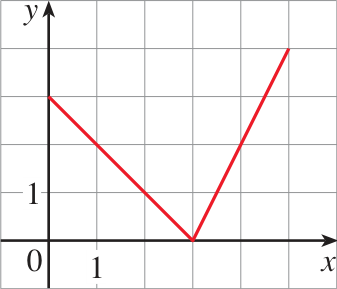
\includegraphics[width=\linewidth]{images/p0055_graph_1.png}}
\hfill
\textbf{64.}\quad \parbox[t]{0.42\linewidth}{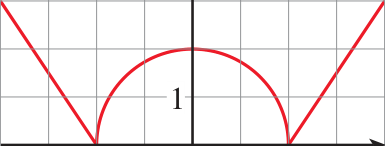
\includegraphics[width=\linewidth]{images/p0055_graph_2.png}}

\vspace{3pt}
\noindent{\color{stewartcyan}\rule{\linewidth}{0.6pt}}
\vspace{3pt}

\noindent
\textbf{\color{stewartcyan}65--70}\quad \textbf{Tìm công thức cho hàm số được mô tả và xác định tập xác định của nó.}

\vspace{2pt}
\noindent
\textbf{65.} Một hình chữ nhật có chu vi $20\text{ m}$. Hãy biểu diễn diện tích của hình chữ nhật dưới dạng một hàm số theo chiều dài một cạnh của nó.

\vspace{2pt}
\noindent
\textbf{66.} Một hình chữ nhật có diện tích $16\text{ m}^2$. Hãy biểu diễn chu vi của hình chữ nhật dưới dạng một hàm số theo chiều dài một cạnh của nó.

\vspace{2pt}
\noindent
\textbf{67.} Biểu diễn diện tích của một tam giác đều dưới dạng một hàm số theo độ dài một cạnh của nó.

\vspace{2pt}
\noindent
\textbf{68.} Một chiếc hộp kín có dạng hình hộp chữ nhật với thể tích $8\text{ ft}^3$ và chiều dài gấp đôi chiều rộng. Hãy biểu diễn chiều cao của chiếc hộp dưới dạng một hàm số theo chiều rộng.

\vspace{2pt}
\noindent
\textbf{69.} Một chiếc hộp không nắp có dạng hình hộp chữ nhật với thể tích $2\text{ m}^3$ và đáy là hình vuông. Hãy biểu diễn diện tích toàn phần của chiếc hộp dưới dạng một hàm số theo độ dài một cạnh đáy.

\vspace{2pt}
\noindent
\textbf{70.} Một hình trụ tròn xoay có thể tích $25\text{ in}^3$. Hãy biểu diễn bán kính của hình trụ dưới dạng một hàm số theo chiều cao của nó.

\vspace{3pt}
\noindent{\color{stewartcyan}\rule{\linewidth}{0.6pt}}
\vspace{3pt}

\noindent
\textbf{71.} Một chiếc hộp không nắp được tạo thành từ một tấm bìa các-tông hình chữ nhật có kích thước $12\text{ in.}$ nhân $20\text{ in.}$ bằng cách cắt bỏ các hình vuông bằng nhau có cạnh $x$ ở bốn góc rồi gấp các mép lên như trong hình vẽ. Hãy biểu diễn thể tích $V$ của chiếc hộp dưới dạng một hàm số theo $x$.

\par\vspace{2pt}{\centering
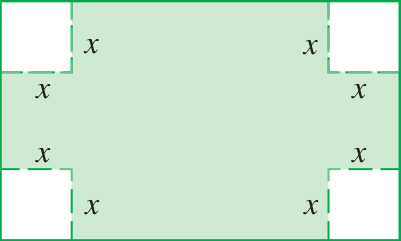
\includegraphics[width=0.44\linewidth]{images/p0055_graph_3.png}\hfill

\includegraphics[width=0.32\linewidth]{images/p0055_graph_4.png}\par}

\vspace{2pt}
\noindent
\textbf{72.} Một cửa sổ kiểu Norman có hình dạng gồm một hình chữ nhật phía trên có một nửa hình tròn gắn vào. Nếu chu vi của cửa sổ là $30\text{ ft}$, hãy biểu diễn diện tích $A$ của cửa sổ dưới dạng một hàm số theo chiều rộng $x$ của nó.

\par\vspace{2pt}{\centering

\includegraphics[width=0.38\linewidth]{images/p0055_graph_5.png}\par}

\end{multicols}